\documentclass[12pt]{article}
\usepackage[a4paper, margin=1in]{geometry} 
\usepackage{graphicx} 
\usepackage{hyperref}
\usepackage{float}
\usepackage[font=small, labelfont=bf]{caption}

\title{Lecture Notes for \\ INF281 Basics of Bioinformatics Sequence Analysis}
\author{Takaya Saito}
\date{}

\begin{document}

\clearpage\maketitle
\vspace{500px}

\includegraphics[scale=1]{fig00/88x31.png} \\
This work is licensed under a Creative Commons Attribution 4.0 International License.
\thispagestyle{empty}
\pagebreak

\pagenumbering{roman}
\setcounter{page}{1}
\tableofcontents
\pagebreak

\pagenumbering{arabic}
\setcounter{page}{1}

%
% PART I
%
\part{}

%
% Introduction
%
\section{Introduction}

%
% Introduction to Molecular Biology
%
\setcounter{figure}{0}
\makeatletter 
\renewcommand{\thefigure}{\arabic{section}.\arabic{figure}}
\makeatother
\subsection{Introduction to Molecular Biology}
Molecular biology is the study of biology focusing on organisms and cells at the molecular level.

\subsubsection*{Five essential facts about cells}

\textbf{1. Two primary types of cells –- eukaryotes and prokaryotes}
\begin{itemize}
\item Eukaryote: animals \& plants
\item Prokaryote: bacteria \& archaea
\end{itemize}
\begin{figure}[H]
  \centering
      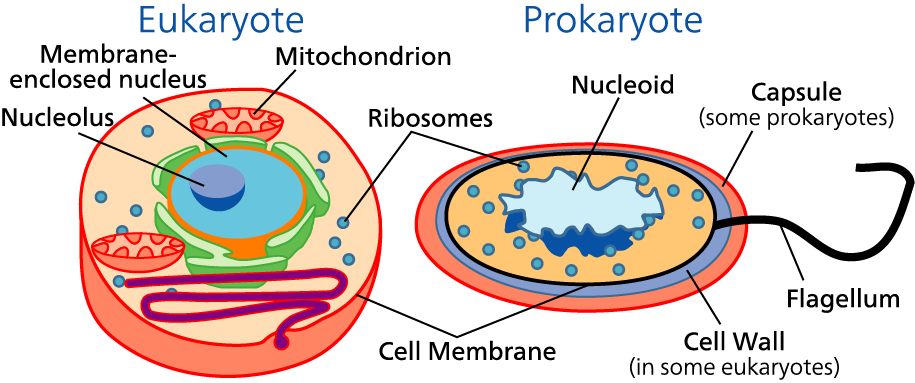
\includegraphics[width=0.75\textwidth]{fig01/prokaryote_and_eukaryote_cells.png}
  \caption{Eukaryotic and prokaryotic cells (source: \href{https://commons.wikimedia.org/wiki/File:Celltypes.svg}{Wikipeida})}
\end{figure}

\noindent \textbf{2. Cell size –- around 1 to 100 micrometers}
\begin{itemize}
\item Cell Size and Scale: \url{http://learn.genetics.utah.edu/content/cells/scale}
\end{itemize}
\medskip  

\noindent \textbf{3. The number of cells}
\begin{itemize}
\item Prokaryotes: 1 cell
\item Human:  Estimate of 15 trillion cells
\end{itemize}
\medskip 

\noindent \textbf{4. An animal cell and cell organelles}
\begin{figure}[H]
  \centering
      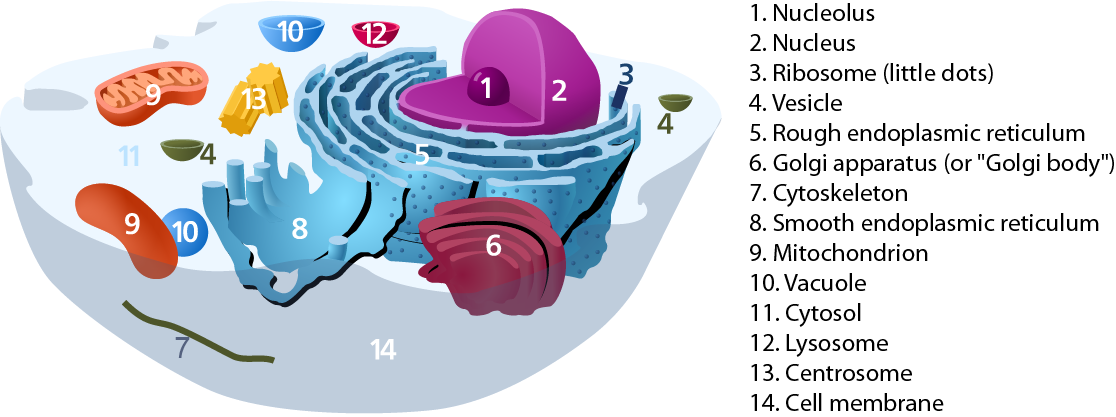
\includegraphics[width=0.75\textwidth]{fig01/animal_cells_and_organelles.png}
  \caption{An animal cell and organelles (source:  \href{https://en.wikipedia.org/wiki/Organelle\#/media/File:Animal_Cell.svg}{Kelvinsong, Wikipedia})}
\end{figure}

\noindent \textbf{5. Cellular processes}
\begin{itemize}
\item Cell growth, cell development, cell signaling, …
\item Example: \url{http://www.nature.com/nrg/multimedia/rnai}
\end{itemize}

\end{document}


